\documentclass[a4paper, 12pt]{article}

\newcommand\tab[1][.6cm]{\hspace*{#1}}
\usepackage[portuges]{babel}
\usepackage[utf8]{inputenc}
\usepackage{amsmath}
\usepackage{indentfirst}
\usepackage{graphicx}
\usepackage{multicol,lipsum}
\usepackage{blindtext}
\usepackage{verbatim}
\usepackage{textcomp}
\usepackage{hyperref}
\usepackage{float}
\usepackage{url}

\begin{document}
%\maketitle

\begin{titlepage}
	\begin{center}
	
	\begin{figure}[ht]
    \centering
    
\includegraphics[width=.44\textwidth]{Images/LogoUFSJ.PNG}
    \label{fig:Capturar.PNG}
    \end{figure}

    	\Huge{Universidade Federal São João del Rei}\\
		\Large{Curso de Ciência da Computação}\\ 

        \vspace{110pt}
        \textbf{\LARGE{
        \\
        \\
        \\
        Trabalho Prático 1 - Parte 2\\
        Relatório\\
        \vspace{0.5cm}
        \Large{Conceitos de Linguagens de Programação}
        \\
        \\
        \\
        }}
        
		\title{{\large{Título}}}
		\vspace{2cm}
	\end{center}
	    
    \begin{flushleft}
		\begin{tabbing}
		\\
		\\
		\\	
		\large{Aluno: Julio Cesar da Silva Rodrigues}\\
	    \\
		\large{Docente: Dárlinton Barbosa Feres Carvalho}\\
	    \end{tabbing}
    \end{flushleft}
	\vspace{0.8cm}
	
	\begin{center}
		\vspace{\fill}
			Outubro\\
		    2022
	\end{center}
\end{titlepage}

\tableofcontents
\newpage
\section{Introdução}

Nesta seção, será apresentada uma breve introdução sobre a proposta do trabalho prático, e o que será abordado mais adiante neste relatório.

\subsection{Contexto}

Os primeiros registros de linguagens de programação surgiram na década de 50 com a \emph{Fortran}. Desde então, com o avanço na área da tecnologia da informação, fez-se necessária a criação de novas linguagens com diversos propósitos de aplicação, assim como a criação de novos paradigmas de programação. Novas formas de pensar foram surgindo, de desenvolver o raciocínio na proposição de soluções para problemas, tudo isto disposto nas mais distintas formas observadas no código fonte, cada uma com suas peculiaridades em relação à vantagens e desvantagens.

\subsection{Descrição do Trabalho}

Neste trabalho, a proposta central é apresentar de forma breve e objetiva, as particularidades envolvidas na utilização de paradigmas de linguagens de programação distintos. Serão apresentadas as soluções desenvolvidas, e também uma análise superficial sobre vantagens e desvantagens encontradas não só no desenvolvimento de tais soluções, mas em aspectos gerais sobre cada paradigma de programação.

\section{Materiais e Métodos}

Nesta seção, serão apresentadas de forma breve as linguagens utilizadas no desenvolvimento de uma solução para o problema, assim como as estratégias aplicadas em cada uma, de acordo com os paradigmas de programação particulares à cada uma delas.

\subsection{Linguagens}

Como sugerido na especificação deste trabalho prático, ao todo foram utilizadas três linguagens de programação distintas: \emph{Python}, \emph{Prolog} e \emph{Haskell}. Estas possuem como base, três paradigmas de programação diferentes: paradigma imperativo (embora \emph{Python} seja uma linguagem multiparadigma, esta foi utilizada de forma imperativa no desenvolvimento da solução para este problema), paradigma lógico e paradigma funcional, respectivamente.

\emph{Python} é uma linguagem de programação de propósito geral, ou seja, pode ser utilizada em diversos tipos de aplicações. Possui abstrações de altíssimo nível e versatilidade com sua sintaxe moderna e objetiva que produz códigos bastante enxutos.

\emph{Prolog} é uma linguagem declarativa, onde geralmente são fornecidas descrições dos problemas à serem resolvidos, utilzando como recursos base, fatos e regras. Possui como fundamentos básicos a lógica de 1ª ordem, o que a torna mais voltada ao conhecimento e sua representação. Com o intuito de obter informação, são realizadas consultas (\emph{queries}) que são computadas por um motor de inferência lógica.

\emph{Haskell} é uma linguagem puramente funcional de propósito geral, que fornece abstrações de altíssimo nível por meio do conceito da utilização de funções da própria matemática na construção de programas no formato do cálculo \emph{lambda}. Entre suas características mais relevantes, se destacam a ausência de efeitos colaterais e a avaliação preguiçosa.

\subsection{Estratégias de Solução}

Inicialmente, foram aplicadas as mesmas estratégias de solução utilizando as três linguagens, ou seja, foram implementadas recursões triviais para possibilitar aos programas o cálculo de forma incremental e recursiva do n-ésimo termo da sequência de Fibonacci. Dado o termo que se deseja calcular, é sempre chamada de forma recursiva o retorno da adição das duas funções, passando como parâmetro o termo (\(N\)) decrementado em uma e duas unidades, respectivamente. Este processo é repetido até o momento em que se tem o caso base, ou seja, os dois valores que somados equivalem ao primeiro termo da sequência (0 e 1). O modelo da declaração da função e da chamada recursiva são exibidos à seguir:

\begin{center}
    \boxed{\textbf{\large{function fibonacci(n)}}}\vspace{0.5cm}
    \boxed{\textbf{\large{return fibonacci(n - 1) + fibonacci(n - 2)}}}
\end{center}

Posteriormente, foi aplicada uma etapa de refatoração nas soluções. A principal motivação para a aplicação deste processo se deve às limitações presentes em algumas linguagens de programação (principalmente aquelas cujo paradigma é puramente funcional ou lógico). Entre elas podemos citar a menor eficiência na execução de programas e o consumo elevado de memória, aspectos provocados pelas recursões.

Todas as três implementações foram adaptadas, introduzindo recursões em cauda, ou seja, agora a chamada recursiva é a última operação à ser realizada pela função. Isto elimina a necessidade de guardar informações referentes às chamadas anteriores da função na recursão, culminando em menor utilização da memória durante o processo de empilhamento (aliviando a \emph{stack}).

Com isto em mente, a mesma ideia foi aplicada utilizando os três paradigmas de programação. A partir do caso base (0 e 1) que vamos denominar agora como \((a)\) e \((b)\), é chamada a função de forma recursiva de acordo com o termo desejado \(N - 1\) vezes, ou seja, a complexidade referente ao número de chamadas recursivas é relacionada diretamente com a magnitude do termo desejado da sequência ($\mathcal{O}(n)$). 

A chamada recursiva sempre é a última instrução executada pela função, decrementando \(N\) em uma unidade e incrementando \((a)\) e \((b)\) gradualmente. O modelo da declaração da função e da chamada recursiva são exibidos à seguir:

\begin{center}
    \boxed{\textbf{\large{function fibonacci(n, a, b)}}}\vspace{0.5cm}
    \boxed{\textbf{\large{return fibonacci(n - 1, b, a + b)}}}
\end{center}

\section{Resultados e Discussão}

Nesta seção, serão discutidos de forma breve alguns aspectos relacionados aos resultados obtidos no desenvolvimento da solução para o problema, além de uma análise superficial em relação as vantagens e desvantagens de cada paradigma de programação explorado.

\subsection{Implementação}

Conforme citado anteriomente, a implementação da solução foi realizada utilizando três linguagens: \emph{Python} (Figura \ref{fig:exampleFig1}), \emph{Prolog} (Figura \ref{fig:exampleFig2}) e \emph{Haskell} (Figura \ref{fig:exampleFig3}). O desenvolvimento foi auxiliado pelo uso da ferramenta de versionamento \emph{GitHub}, e o código fonte está disponível publicamente em: \url{https://github.com/juliorodrigues07/fibonacci_clp}.

À seguir serão exibidos os \emph{scripts} das soluções finais (com recursão em cauda) implementadas em cada uma das linguagens:

\begin{figure}[H]
    \centering
    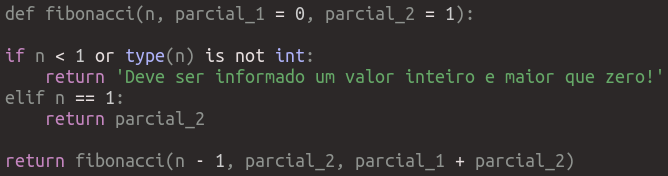
\includegraphics[width=1\textwidth]{Images/python.png}
    \caption{Implementação com Paradigma Imperativo (\emph{Python})}
    \label{fig:exampleFig1}
\end{figure}

\begin{figure}[H]
    \centering
    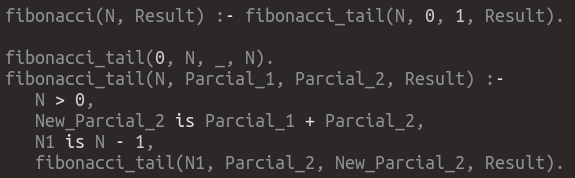
\includegraphics[width=0.82\textwidth]{Images/prolog.png}
    \caption{Implementação com Paradigma Lógico (\emph{Prolog})}
    \label{fig:exampleFig2}
\end{figure}

\begin{figure}[H]
    \centering
    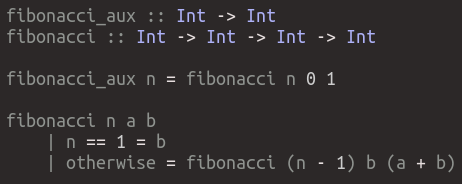
\includegraphics[width=0.75\textwidth]{Images/haskell.png}
    \caption{Implementação com Paradigma Funcional (\emph{Haskell})}
    \label{fig:exampleFig3}
\end{figure}

\subsection{Análise}

Embora todas as implementações tenham gerado código enxuto (problema de simples solução), os paradigmas distintos, somados a sintaxe distante entre as linguagens contribuíram para a construção de código bastante distinto, mas que possuem a mesma ideia principal de solução em seu núcleo. Na próxima subseção, teremos uma visão mais detalhada sobre as particularidades de cada paradigma e linguagem correspondente. 

Mas antes, vamos analisar de forma bastante superficial o desempenho de cada implementação em cada paradigma de linguagem, utilizando como métrica básica o tempo de execução. Para evitar viés em relação à execução em máquinas locais, todas as implementações foram testadas em \emph{IDEs} online: \hyperlink{https://colab.research.google.com/}{Google Colab} (\emph{Python}), \hyperlink{https://swish.swi-prolog.org/}{SWISH} (\emph{Prolog}) e \hyperlink{https://www.codingrooms.com/}{Coding Rooms} (\emph{Haskell}).

Na implementação inicial, ou seja, utilizando a recursão comum, todos os \emph{IDEs} encontraram problemas na execução, principalmente no caso da linguagem \emph{Prolog}, cujos avisos de "estouro" de pilha (0.2 GB) começaram a se apresentar com termos da sequência de \emph{Fibonacci} posteriores ao vigésimo, além do aumento exponencial no tempo de execução observado. Por isto, foi mantido o limite de \(N\) em 20 para executar os programas, obtendo resultados que são sumarizados na Figura \ref{fig:exampleFig4}:

\begin{figure}[H]
    \centering
    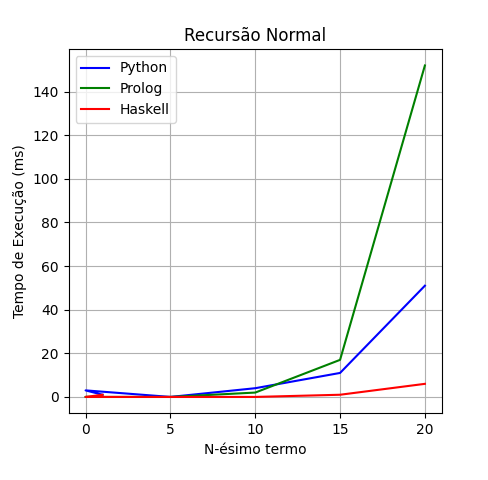
\includegraphics[width=0.75\textwidth]{Images/normal.png}
    \caption{Tempos de execução na recursão normal}
    \label{fig:exampleFig4}
\end{figure}

Na versão aprimorada da solução, ou seja, com a utilização da recursão em cauda, os resultados obtidos foram consideravelmente melhores, embora uma limitação presente na \emph{IDE} para \emph{Haskell} tenha prejudicado os testes com termos de grande magnitude. Os maiores valores representáveis (\emph{maxBound}) são da ordem de \(2^{63}\), o que corresponde à no máximo o 92º termo da sequência de \emph{Fibonacci}, o que limitou os testes com \(N\) até este valor. Por isto, os resultados obtidos não são muito representativos (Figura \ref{fig:exampleFig5}), embora mostrem claramente que a recursão em cauda tem grande impacto no tempo de execução do algoritmo.

\begin{figure}[H]
    \centering
    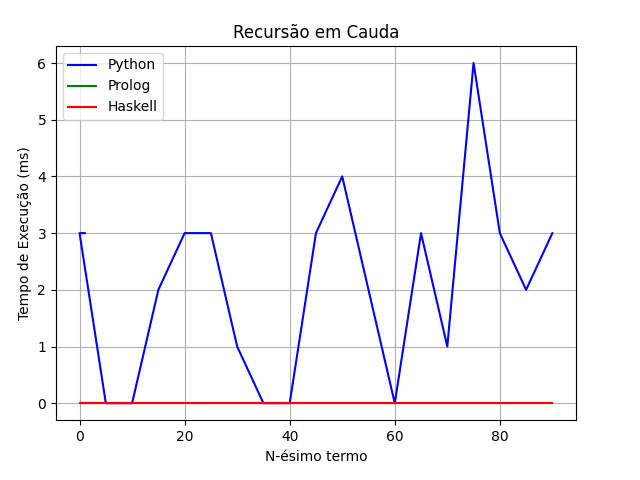
\includegraphics[width=0.95\textwidth]{Images/tail.png}
    \caption{Tempos de execução na recursão em cauda}
    \label{fig:exampleFig5}
\end{figure}

\subsection{Vantagens e Desvantagens}

A inclusão da recursão em cauda, embora possa trazer diversos benefícios para linguagens de programação em geral, julgo que prejudicou aspectos como legibilidade de código. Foi necessário incluir mais parâmetros, a fim de obter os resultados com base no incremento gradual dos valores base. No processo de refatoramento destas soluções, o paradigma em que encontrei maiores obstáculos na compreensão de como formular a solução foi o paradigma lógico, tanto devido à forma bastante distinta de pensar (fatos e regras), quanto à sintaxe da própria linguagem \emph{Prolog}.

A solução implementada em \emph{Haskell}, embora tenha gerado o código menos verboso, com abstrações de altíssimo nível, apresentou alguns empecilhos no desenvolvimento quando comparada à mesma escrita em \emph{Python}. A linguagem \emph{Haskell} não fornece suporte à inserção de parâmetros opcionais para suas funções, o que implicou na criação de uma segunda função auxiliar, que então realiza a chamada da função responsável por calcular o n-ésimo termo da sequência de \emph{Fibonacci}, passando como parâmetros os valores base de \(a\) e \(b\) (0 e 1).

\section{Conclusão}

Neste trabalho, foram exploradas soluções para o cálculo do n-ésimo termo da sequência de \emph{Fibonacci} que possuem a mesma ideia em seu núcleo, mas que foram implementadas de forma distintas, adequando-se aos paradigmas de programação presentes nas linguagens escolhidas, além é claro, de suas sintaxes.

Com este pequeno exemplo didático, podemos observar a exigência de diferentes formas de se pensar quando se deseja trabalhar com paradigmas de linguagens de programação distintos. Embora a maioria destas linguagens possam ser utilizadas para propósito geral, a escolha de uma linguagem para desenvolvimento deve levar em conta diversos fatores referentes aos paradigmas. Níveis de abstração, desempenho, legibilidade, e claro, a forma de raciocínio para a escrita de programas, são aspectos extremamente importantes que devem ser analisados extensamente no desenvolvimento de soluções para problemas de escopo geral.

\section*{Referências}

\begin{itemize}
    \item Optional Parameters in Haskell: \url{https://neilmitchell.blogspot.com/2008/04/optional-parameters-in-haskell.html}
    \item What is Tail Recursion: \url{https://www.geeksforgeeks.org/tail-recursion/}
    \item Introduction of Programming Paradigms: \url{https://www.geeksforgeeks.org/introduction-of-programming-paradigms/}
    \item Fibonacci Series - Recursive or Iterative? Elegance or Speed?: \url{https://groups.google.com/g/comp.lang.prolog/c/r_HO45eyVdc}
    \item Material disponível no portal didático na disciplina de CLP
\end{itemize}

\end{document}
